%\documentclass[10pt, aspectratio=169]{beamer}
\documentclass[10pt,hyperref={colorlinks = true,linkcolor = blue}, aspectratio=169]{beamer}

% handout
% \documentclass[handout, 10pt]{beamer}
\usepackage{clases}

\title{Investigacion Operativa}
\subtitle{Recorrido de grafos y camino mínimo}
\date{}
\author{Facundo Gutiérrez - Nazareno Faillace}
\institute{Departamento de Matemática, FCEN, UBA}
% \titlegraphic{\hfill\includegraphics[height=1.5cm]{logo.pdf}}

\newcommand \anchoPagina{1.0} % El proyector no anda bien, hay que ajustar el ancho
\begin{document}

\maketitle

\begin{frame}{Recorrido de Grafos - BFS}
    \begin{minipage}{\anchoPagina \textwidth}
        Dado un grafo $G = (\mathbb{V},\mathbb{E})$, queremos recorrer sus vértices. En una primera
        instancia vamos a asumir que es \textit{conexo}. Según cómo decidamos recorrer el grafo vamos a poder
        \orangealert{distinguir distintas propiedades estructurales} del mismo.
        \pause
        \vspace{0.3cm}

        En un recorrido \orangealert{BFS} (\textit{Breadth-First Search})
        vamos a distinguir a un nodo en particular donde comenzaremos el
        recorrido del grafo. Llamémosle $s$ a dicho nodo.

        \vspace{0.3cm}
        \pause
        Comenzamos visitando el nodo $s$, luego visitamos a todos los vecinos de $s$ (que son los nodos que están
        a distancia 1 de $s$), después visitamos a los vecinos de estos vecinos (que son los nodos que están
        a distancia 2 de $s$), y así \dots.
    \end{minipage}
\end{frame}

\begin{frame}{Algoritmo BFS}
    A lo largo del algoritmo utilizaremos:
    \pause
    \begin{itemize}
        \item $\mathbb{S}$: indica la capa actual de vértices que estamos visitando.
        \item $\mathbb{W}$: indica la capa siguiente de vértices por visitar.
        \item $\texttt{visto}$: un arreglo auxiliar que indica qué vértices ya fueron procesados.
        \item $s$: vértice inicial en el que comenzamos el recorrido.
    \end{itemize}
\end{frame}

\begin{frame}{Algoritmo BFS}
    BFS($G,s$):
    \begin{enumerate}
        \item $\forall v \in \mathbb{V}:  \texttt{visto}[v] \leftarrow Falso$
        \item
        $\texttt{visto}[s]  \leftarrow Verdadero, \mathbb{S} \leftarrow \{ s \}, \mathbb{W} \leftarrow
        \varnothing$
        \item Mientras $\mathbb{S} \neq \varnothing$:
        \begin{enumerate}
            \item $\forall v \in \mathbb{S}: $
            \begin{enumerate}
                \item $\forall w \in \{ u \in \mathcal{N}(v) : \texttt{visto}[u] = Falso \}$:

                \item [] \quad Agregar $w$ a $\mathbb{W}$
                \item [] \quad $\texttt{visto}[w] \leftarrow Verdadero$

            \end{enumerate}
            \item $\mathbb{S} \leftarrow \mathbb{W}$
            \item $\mathbb{W} \leftarrow \varnothing$
        \end{enumerate}
    \end{enumerate}
    \pause
    ¿Cómo podemos modificarlo para \orangealert{calcular la distancia} a $s$?
\end{frame}

\begin{frame}{Recorrido de Grafos - BFS}
    \begin{minipage}{\anchoPagina \textwidth}
        \begin{center}
            \includegraphics<1>[scale = 0.45]{imagenes/bfs-1.png}%
            \includegraphics<2>[scale = 0.45]{imagenes/bfs-2.png}%
            \includegraphics<3>[scale = 0.45]{imagenes/bfs-3.png}%
            \includegraphics<4>[scale = 0.45]{imagenes/bfs-4.png}%
            \includegraphics<5>[scale = 0.45]{imagenes/bfs-5.png}%
            \includegraphics<6>[scale = 0.45]{imagenes/bfs-6.png}%
        \end{center}
    \end{minipage}
\end{frame}

\begin{frame}{Recorrido de Grafos - BFS}
    \begin{minipage}{\anchoPagina \textwidth}
        \begin{center}
            \includegraphics<1>[scale = 0.45]{imagenes/maze-bfs-1.png}%
            \includegraphics<2>[scale = 0.45]{imagenes/maze-bfs-2.png}%
            \includegraphics<3>[scale = 0.45]{imagenes/maze-bfs-3.png}%
            \includegraphics<4>[scale = 0.45]{imagenes/maze-bfs-4.png}%
            \includegraphics<5>[scale = 0.45]{imagenes/maze-bfs-5.png}%
            \includegraphics<6>[scale = 0.45]{imagenes/maze-bfs-6.png}%
            \includegraphics<7>[scale = 0.45]{imagenes/maze-bfs-7.png}%
            \includegraphics<8>[scale = 0.45]{imagenes/maze-bfs-8.png}%
            \includegraphics<9>[scale = 0.45]{imagenes/maze-bfs-9.png}%
            \includegraphics<10>[scale = 0.45]{imagenes/maze-bfs-10.png}%
            \includegraphics<11>[scale = 0.45]{imagenes/maze-bfs-11.png}%
            \includegraphics<12>[scale = 0.45]{imagenes/maze-bfs-12.png}%
            \includegraphics<13>[scale = 0.45]{imagenes/maze-bfs-13.png}%
            \includegraphics<14>[scale = 0.45]{imagenes/maze-bfs-14.png}%
            \includegraphics<15>[scale = 0.45]{imagenes/maze-bfs-15.png}%
            \includegraphics<16>[scale = 0.45]{imagenes/maze-bfs-16.png}%
            \includegraphics<17>[scale = 0.45]{imagenes/maze-bfs-17.png}%
            \includegraphics<18>[scale = 0.45]{imagenes/maze-bfs-18.png}%
            \includegraphics<19>[scale = 0.45]{imagenes/maze-bfs-19.png}%
            \includegraphics<20>[scale = 0.45]{imagenes/maze-bfs-20.png}%
            \includegraphics<21>[scale = 0.45]{imagenes/maze-bfs-21.png}%
            \includegraphics<22>[scale = 0.45]{imagenes/maze-bfs-22.png}%
            \includegraphics<23>[scale = 0.45]{imagenes/maze-bfs-23.png}%
            \includegraphics<24>[scale = 0.45]{imagenes/maze-bfs-24.png}%
            \includegraphics<25>[scale = 0.45]{imagenes/maze-bfs-25.png}%
            \includegraphics<26>[scale = 0.45]{imagenes/maze-bfs-26.png}%
            \includegraphics<27>[scale = 0.45]{imagenes/maze-bfs-27.png}%
            \includegraphics<28>[scale = 0.45]{imagenes/maze-bfs-28.png}%
            \includegraphics<29>[scale = 0.45]{imagenes/maze-bfs-29.png}%
            \includegraphics<30>[scale = 0.45]{imagenes/maze-bfs-30.png}%
        \end{center}
    \end{minipage}
\end{frame}

\begin{frame}{Recorrido de Grafos - BFS}
    \begin{minipage}{\anchoPagina \textwidth}
        Cada nodo se agrega a lo sumo una vez a $\mathbb{S}$. Cuando procesamos a un nodo en $\mathbb{S}$
        analizamos la situación de todos sus vecinos. Por lo tanto, en total \orangealert{hacemos
            $\mathcal{O}(|\mathbb{V}| + |\mathbb{E}|)$} operaciones (lo cual es lineal en el grafo).
        \pause

        Adem\'as de simplemente recorrer un grafo en general, los usos m\'as comunes de BFS (o alguna modificaci\'
        on del mismo) involucran:
        \pause
        \begin{itemize}
            \item Calcular distancias desde una fuente
            \pause
            \item Chequear si un cierto grafo es bipartito
            \pause
            \item Calcular componentes conexas
        \end{itemize}
        \pause
        ¿Qué podemos hacer si el grafo no es \textit{conexo}?
    \end{minipage}
\end{frame}

\begin{frame}{Recorrido de Grafos - DFS}
    \begin{minipage}{\anchoPagina \textwidth}
        Veamos otra forma de recorrer a $G = (\mathbb{V},\mathbb{E})$
        de una forma que ya fuimos utilizando a lo largo de la materia (por ejemplo en Branch \& Bound).
        \pause

        Vamos a distinguir a un nodo en particular que indica el nodo actual del recorrido. Llamémosle $v$
        a dicho nodo.

        \pause
        En un recorrido \orangealert{DFS} (\textit{Depth-First Search}) comenzamos visitando el nodo $v$
        , luego visitamos a alg\'un vecino y seguimos un recorrido DFS desde allí. As\'
        i hasta que todos los vecinos de $v$ sean visitados. Una vez que todos los vecinos de $v$ están
        visitados, se da por finalizado el recorrido desde $v$.
        \pause

        De alguna forma, podemos pensar que se va expandiendo ordenadamente en una dirección todo lo que puede.

    \end{minipage}

\end{frame}



\begin{frame}{Algoritmo DFS}
    \begin{minipage}{\anchoPagina \textwidth}
        Por la naturaleza del algoritmo, las implementaciones usuales del recorrido DFS de un grafo son recursivas.
        A lo largo del algoritmo utilizaremos el arreglo auxiliar $\texttt{visto}$ de manera similar.
    \end{minipage}
\end{frame}

\begin{frame}{Algoritmo DFS}
    DFS($G$):
    \begin{enumerate}
        \item $\forall v \in \mathbb{V}: \texttt{visto}[v] \leftarrow Falso$
        \item $\forall v \in \mathbb{V}: \text{Si } \texttt{visto}[v] = Falso:$
        \begin{enumerate}
            \item DFS-VISITA($G,v, \texttt{visto}$)
        \end{enumerate}
    \end{enumerate}
    \pause

    DFS-VISITA($G,v, \texttt{visto}$):
    \begin{enumerate}
        \item $\texttt{visto}[v] \leftarrow Verdadero$
        \item $\forall w \in \{u \in N(v) : \texttt{visto}[u] = Falso \}$
        \begin{enumerate}
            \item DFS-VISITA($G,w, \texttt{visto}$)
        \end{enumerate}
    \end{enumerate}
    \pause

    ¿Cómo podemos modificarlo para encontrar la cantidad de componentes conexas del grafo?
\end{frame}

\begin{frame}{Recorrido de Grafos - DFS}
    \begin{minipage}{\anchoPagina \textwidth}
        \begin{center}
            \includegraphics<1>[scale = 0.45]{imagenes/dfs-1.png}%
            \includegraphics<2>[scale = 0.45]{imagenes/dfs-2.png}%
            \includegraphics<3>[scale = 0.45]{imagenes/dfs-3.png}%
            \includegraphics<4>[scale = 0.45]{imagenes/dfs-4.png}%
            \includegraphics<5>[scale = 0.45]{imagenes/dfs-5.png}%
            \includegraphics<6>[scale = 0.45]{imagenes/dfs-6.png}%
            \includegraphics<7>[scale = 0.45]{imagenes/dfs-7.png}%
            \includegraphics<8>[scale = 0.45]{imagenes/dfs-8.png}%
            \includegraphics<9>[scale = 0.45]{imagenes/dfs-9.png}%
            \includegraphics<10>[scale = 0.45]{imagenes/dfs-10.png}%
            \includegraphics<11>[scale = 0.45]{imagenes/dfs-11.png}%
            \includegraphics<12>[scale = 0.45]{imagenes/dfs-12.png}%
            \includegraphics<13>[scale = 0.45]{imagenes/dfs-13.png}%
            \includegraphics<14>[scale = 0.45]{imagenes/dfs-14.png}%
            \includegraphics<15>[scale = 0.45]{imagenes/dfs-15.png}%
            \includegraphics<16>[scale = 0.45]{imagenes/dfs-16.png}%
            \includegraphics<17>[scale = 0.45]{imagenes/dfs-17.png}%
            \includegraphics<18>[scale = 0.45]{imagenes/dfs-18.png}%
            \includegraphics<19>[scale = 0.45]{imagenes/dfs-19.png}%
            \includegraphics<20>[scale = 0.45]{imagenes/dfs-20.png}%
            \includegraphics<21>[scale = 0.45]{imagenes/dfs-21.png}%
            \includegraphics<22>[scale = 0.45]{imagenes/dfs-22.png}%
            \includegraphics<23>[scale = 0.45]{imagenes/dfs-23.png}%
        \end{center}
    \end{minipage}
\end{frame}

\begin{frame}{Recorrido de Grafos - DFS}
    \begin{minipage}{\anchoPagina \textwidth}
        \centering
        \begin{center}
            \includegraphics<1>[scale = 0.45]{imagenes/maze-dfs-1.png}%
            \includegraphics<2>[scale = 0.45]{imagenes/maze-dfs-2.png}%
            \includegraphics<3>[scale = 0.45]{imagenes/maze-dfs-3.png}%
            \includegraphics<4>[scale = 0.45]{imagenes/maze-dfs-4.png}%
            \includegraphics<5>[scale = 0.45]{imagenes/maze-dfs-5.png}%
            \includegraphics<6>[scale = 0.45]{imagenes/maze-dfs-6.png}%
            \includegraphics<7>[scale = 0.45]{imagenes/maze-dfs-7.png}%
            \includegraphics<8>[scale = 0.45]{imagenes/maze-dfs-8.png}%
            \includegraphics<9>[scale = 0.45]{imagenes/maze-dfs-9.png}%
            \includegraphics<10>[scale = 0.45]{imagenes/maze-dfs-10.png}%
            \includegraphics<11>[scale = 0.45]{imagenes/maze-dfs-11.png}%
            \includegraphics<12>[scale = 0.45]{imagenes/maze-dfs-12.png}%
            \includegraphics<13>[scale = 0.45]{imagenes/maze-dfs-13.png}%
            \includegraphics<14>[scale = 0.45]{imagenes/maze-dfs-14.png}%
            \includegraphics<15>[scale = 0.45]{imagenes/maze-dfs-15.png}%
            \includegraphics<16>[scale = 0.45]{imagenes/maze-dfs-16.png}%
            \includegraphics<17>[scale = 0.45]{imagenes/maze-dfs-17.png}%
            \includegraphics<18>[scale = 0.45]{imagenes/maze-dfs-18.png}%
            \includegraphics<19>[scale = 0.45]{imagenes/maze-dfs-19.png}%
            \includegraphics<20>[scale = 0.45]{imagenes/maze-dfs-20.png}%
            \includegraphics<21>[scale = 0.45]{imagenes/maze-dfs-21.png}%
            \includegraphics<22>[scale = 0.45]{imagenes/maze-dfs-22.png}%
            \includegraphics<23>[scale = 0.45]{imagenes/maze-dfs-23.png}%
            \includegraphics<24>[scale = 0.45]{imagenes/maze-dfs-24.png}%
            \includegraphics<25>[scale = 0.45]{imagenes/maze-dfs-25.png}%
            \includegraphics<26>[scale = 0.45]{imagenes/maze-dfs-26.png}%
            \includegraphics<27>[scale = 0.45]{imagenes/maze-dfs-27.png}%
            \includegraphics<28>[scale = 0.45]{imagenes/maze-dfs-28.png}%
            \includegraphics<29>[scale = 0.45]{imagenes/maze-dfs-29.png}%
            \includegraphics<30>[scale = 0.45]{imagenes/maze-dfs-30.png}%
            \includegraphics<31>[scale = 0.45]{imagenes/maze-dfs-31.png}%
            \includegraphics<32>[scale = 0.45]{imagenes/maze-dfs-32.png}%
            \includegraphics<33>[scale = 0.45]{imagenes/maze-dfs-33.png}%
            \includegraphics<34>[scale = 0.45]{imagenes/maze-dfs-34.png}%
            \includegraphics<35>[scale = 0.45]{imagenes/maze-dfs-35.png}%
            \includegraphics<36>[scale = 0.45]{imagenes/maze-dfs-36.png}%
            \includegraphics<37>[scale = 0.45]{imagenes/maze-dfs-37.png}%
            \includegraphics<38>[scale = 0.45]{imagenes/maze-dfs-38.png}%
            \includegraphics<39>[scale = 0.45]{imagenes/maze-dfs-39.png}%
            \includegraphics<40>[scale = 0.45]{imagenes/maze-dfs-40.png}%
            \includegraphics<41>[scale = 0.45]{imagenes/maze-dfs-41.png}%
            \includegraphics<42>[scale = 0.45]{imagenes/maze-dfs-42.png}%
            \includegraphics<43>[scale = 0.45]{imagenes/maze-dfs-43.png}%
            \includegraphics<44>[scale = 0.45]{imagenes/maze-dfs-44.png}%
            \includegraphics<45>[scale = 0.45]{imagenes/maze-dfs-45.png}%
            \includegraphics<46>[scale = 0.45]{imagenes/maze-dfs-46.png}%
            \includegraphics<47>[scale = 0.45]{imagenes/maze-dfs-47.png}%
            \includegraphics<48>[scale = 0.45]{imagenes/maze-dfs-48.png}%
        \end{center}
    \end{minipage}
\end{frame}

\begin{frame}{Recorrido de Grafos - DFS}
    \begin{minipage}{\anchoPagina \textwidth}
        Notemos que DFS-VISITA se llama solo si $\texttt{visto}[v] = Falso$ e inmediatamente después se tiene que
        $\texttt{visto}[v] = Verdadero$ (por cómo funciona el algoritmo), por lo tanto se hacen a lo sumo
        $\mathcal{O}(|\mathbb{V}|)$ llamadas a DFS-VISITA.
        \pause
        \vspace{0.3cm}

        Adem\'as, por cada llamada a DFS-VISITA, debemos analizar la situaci\'
        on de todos sus vecinos. Por lo tanto, \orangealert{la complejidad temporal del algoritmo nos queda
            $\mathcal{O}(|\mathbb{V}| + |\mathbb{E}|)$}
    \end{minipage}
\end{frame}

\begin{frame}{Recorrido de Grafos - DFS}
    Algunos usos del algoritmo DFS para obtener información estructural del grafo incluyen:
    \begin{itemize}
        \item Componentes conexas
        \item Puentes, puntos de corte, componentes biconexas
        \item Componentes fuertemente conexas
%            \item Orden topológico en DAGs.
    \end{itemize}
\end{frame}

\begin{frame}{Ejercicio 1}
    \begin{minipage}{\anchoPagina \textwidth}
        Calcular el n\'umero Erd\H{o}s de Willy, ¿Qué algoritmo usaríamos y cómo lo usaríamos?
        \begin{center}
            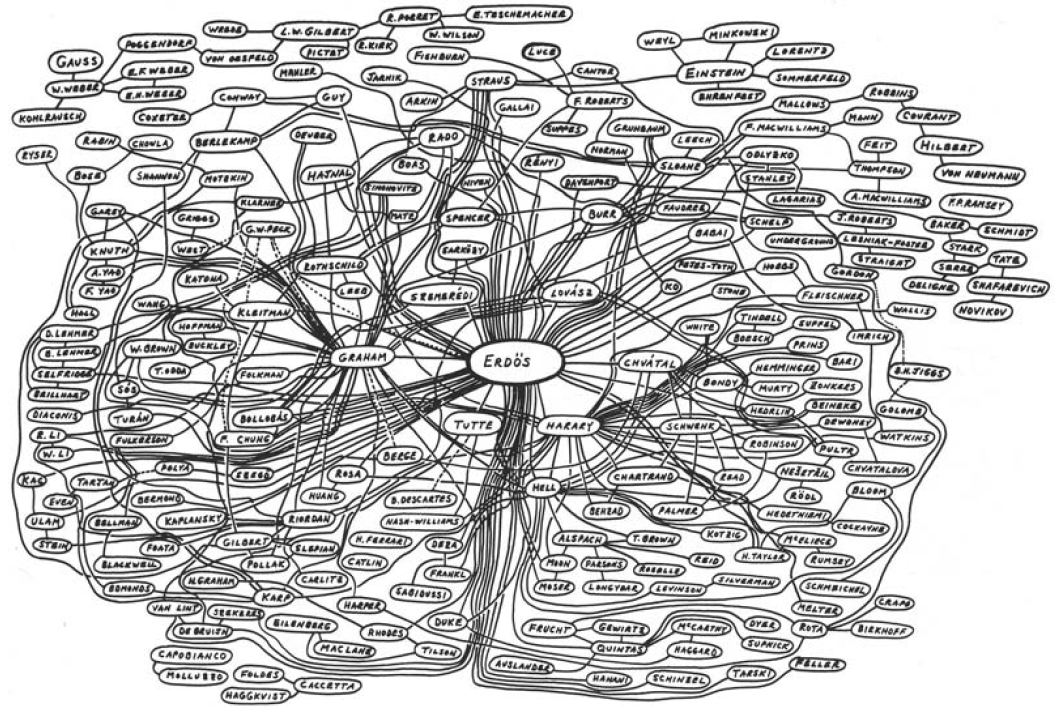
\includegraphics[scale = 0.28]{imagenes/erdos.png}
        \end{center}
    \end{minipage}
\end{frame}

\begin{frame}{Ejercicio 2}
    \begin{minipage}{\anchoPagina \textwidth}
        Supongamos que tenemos un Trie en el que están
        a almacenado un conjunto de palabras y se nos pide que demos el listado de palabras que hay en el
        diccionario en orden lexicogr\'afico. ¿Qué algoritmo usaríamos y cómo lo usaríamos?
        \begin{center}
            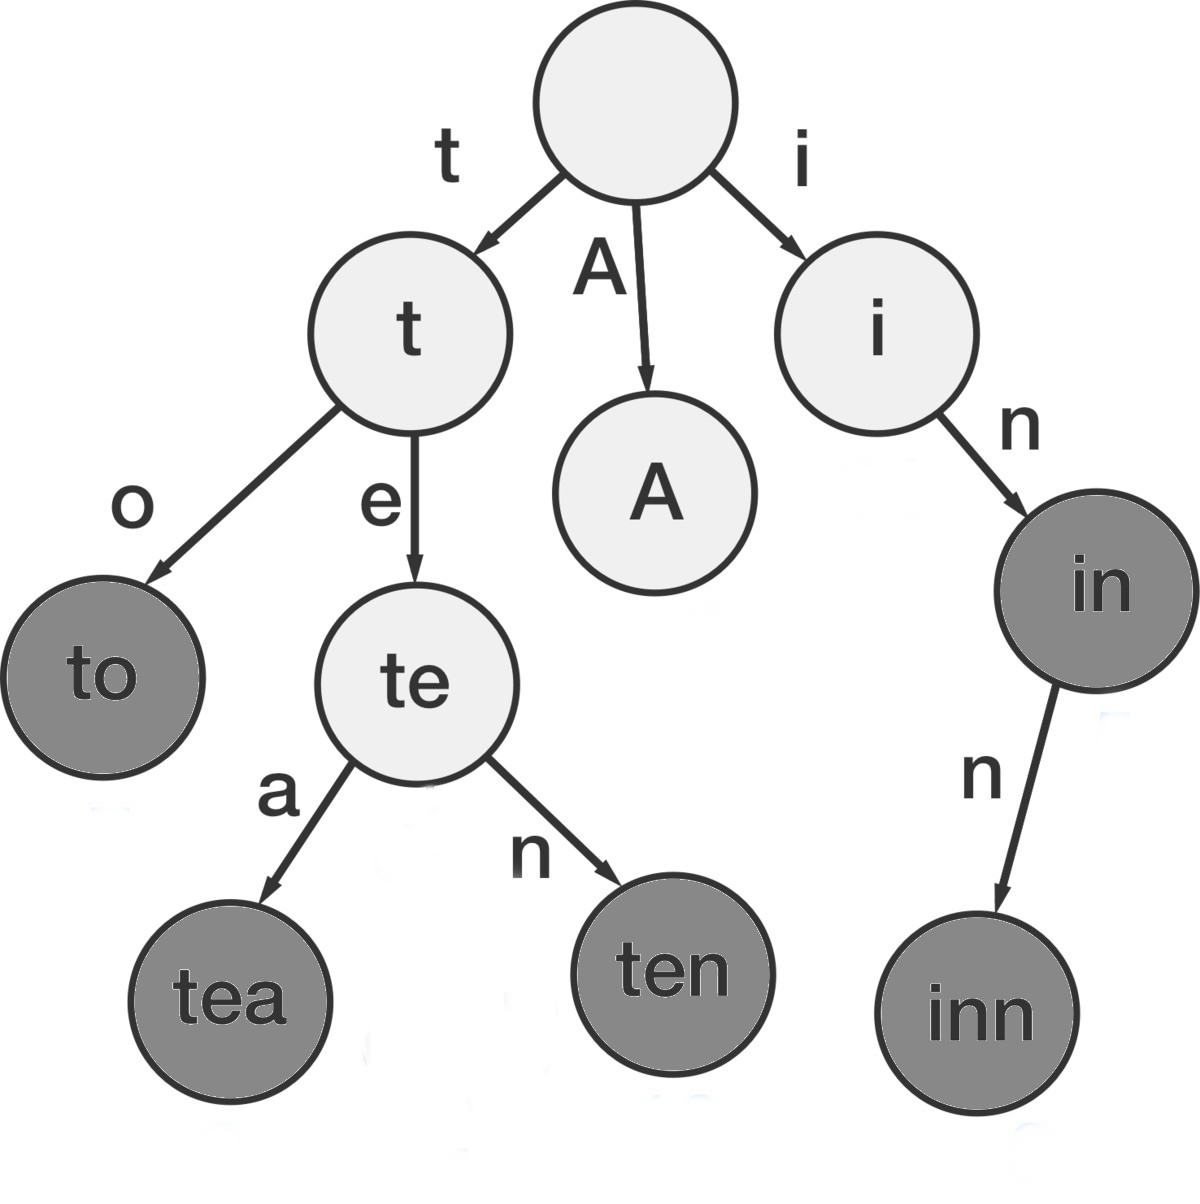
\includegraphics[scale = 0.15]{imagenes/Trie.jpg}
        \end{center}
    \end{minipage}
\end{frame}

%    \begin{frame}{Grafos Dirigidos Acíclicos (DAG) - Orden Topológico}
%        \begin{minipage}{\anchoPagina \textwidth}
%            \begin{center}
%                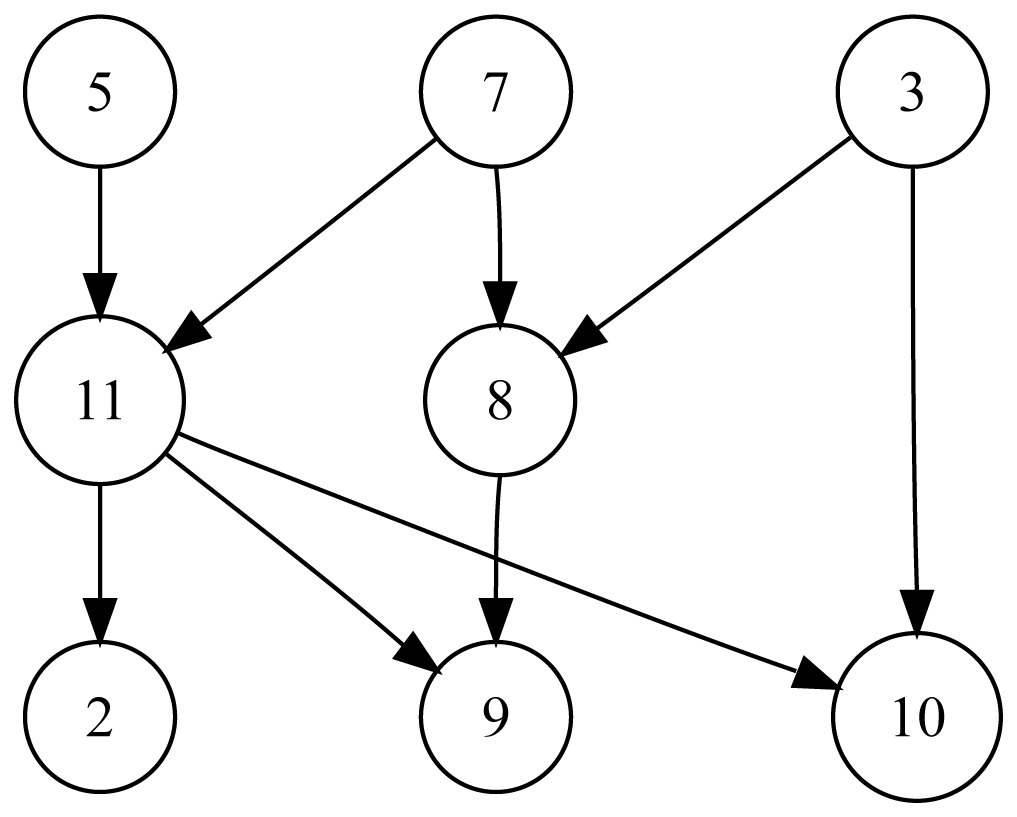
\includegraphics[scale = 0.5]{imagenes/dag.jpg}
%            \end{center}
%            \pause
%            \medskip
%            \medskip
%            \medskip
%            \begin{center}
%                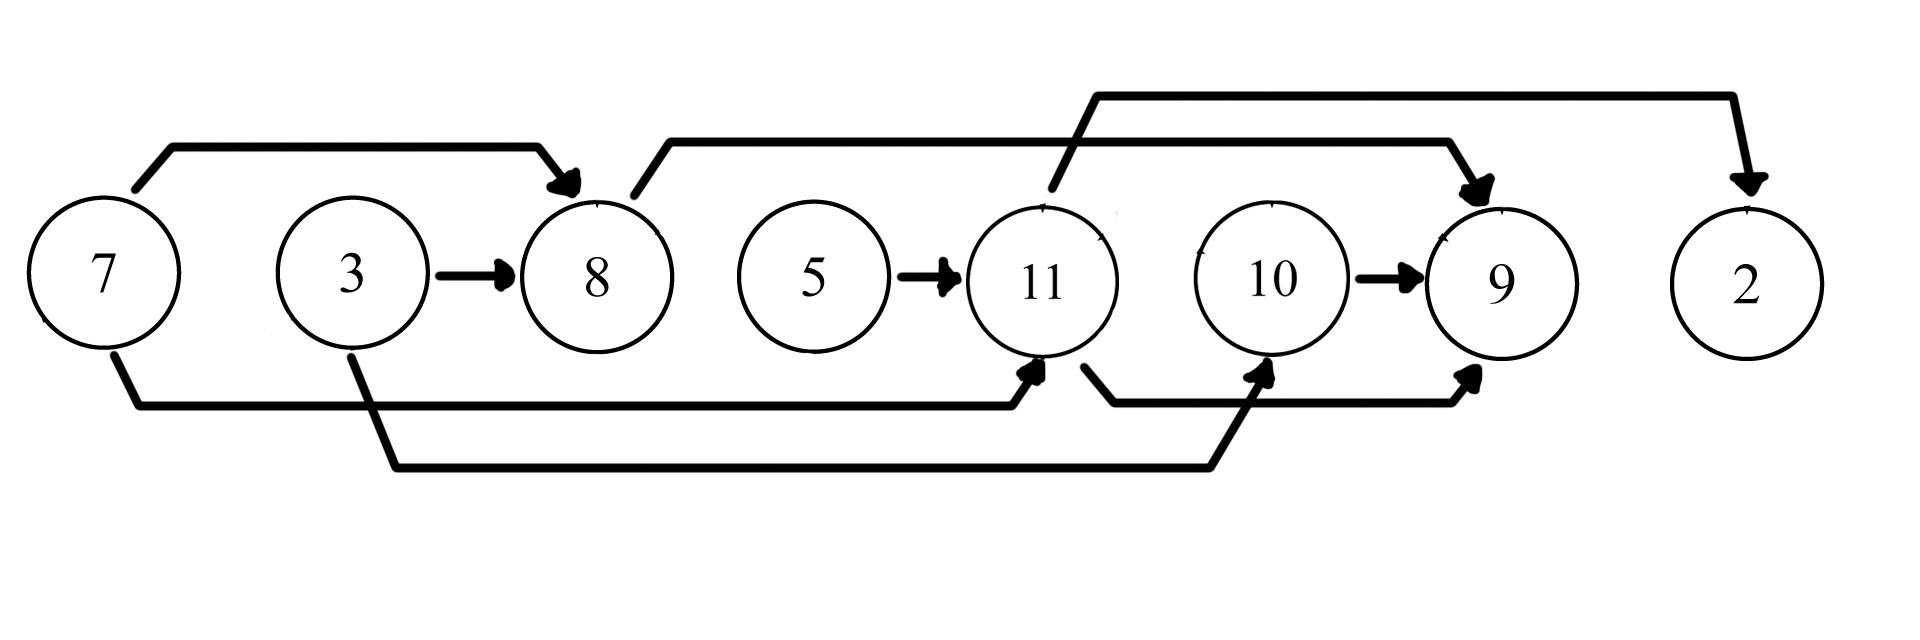
\includegraphics[scale = 0.35]{imagenes/dagorder.jpg}
%            \end{center}
%        \end{minipage}
%    \end{frame}

\begin{frame}{Caminos mínimos}
    \begin{tcolorbox}[colbacktitle=YellowOrange, coltitle=black, title=Definición]
        $G=(V,A,\omega)$ es un digrafo pesado, donde $V$ es el conjunto de vértices, $A$ el conjunto de arcos
        y $\omega$ una función tal que $\omega\colon\, A\rightarrow \mathbb{R}$.
    \end{tcolorbox}

    \centering
    \begin{tikzpicture}
        \tikzstyle{normal}=[fill=white, draw=black, shape=circle];
        \tikzstyle{directed}=[-Latex];

        \node[normal] (C) at (0,0) {$C$};
        \node[normal] (D) at (2,0) {$D$};
        \node[normal] (E) at (4,0) {$E$};
        \node[normal] (A) at (1,2) {$A$};
        \node[normal] (B) at (3,2) {$B$};

        \draw[directed] (C) to node[midway,below]{$8$} (D) ;
        \draw[directed] (A) to node[midway,left]{$5$} (C) ;
        \draw[directed] (D) to node[midway,below]{$-3$} (E) ;
        \draw[directed] (B) to node[midway,right]{$0$} (D) ;
        \draw[directed] (A) to node[midway,left]{$\frac{3}{2}$} (D) ;
        \draw[directed] (A) to node[midway,above]{$1$} (B) ;
    \end{tikzpicture}
\end{frame}

\begin{frame}{Caminos Mínimos}
    \begin{columns}
        \begin{column}{0.5\textwidth}
            \centering
            \begin{tikzpicture}
                \tikzstyle{normal}=[fill=white, draw=black, shape=circle];
                \tikzstyle{directed}=[-Latex];

                \node[normal] (C) at (0,0) {$C$};
                \node[normal] (D) at (2,0) {$D$};
                \node[normal] (E) at (4,0) {$E$};
                \node[normal] (A) at (1,2) {$A$};
                \node[normal] (B) at (3,2) {$B$};

                \draw[directed] (C) to node[midway,below]{$1$} (D) ;
                \draw[directed] (A) to node[midway,left]{$1$} (C) ;
                \draw[directed] (D) to node[midway,below]{$1$} (E) ;
                \draw[directed] (B) to node[midway,right]{$1$} (D) ;
                \draw[directed] (A) to node[midway,left]{$1$} (D) ;
                \draw[directed] (A) to node[midway,above]{$1$} (B) ;
            \end{tikzpicture}
        \end{column}
        \begin{column}{0.5\textwidth}
            Para este grafo pesado, ¿qué algoritmo podemos usar para calcular el \orangealert{camino mínimo} desde
            $A$ al resto de los vértices?
            \pause
            \vspace{1cm}

            \orangealert{BFS} {\small con una pequeña modificación}
        \end{column}
    \end{columns}
\end{frame}

\begin{frame}{Caminos Mínimos}
    \begin{columns}
        \begin{column}{0.5\textwidth}
            \centering
            \begin{tikzpicture}
                \tikzstyle{normal}=[fill=white, draw=black, shape=circle];
                \tikzstyle{directed}=[-Latex];

                \node[normal] (C) at (0,0) {$C$};
                \node[normal] (D) at (2,0) {$D$};
                \node[normal] (E) at (4,0) {$E$};
                \node[normal] (A) at (1,2) {$A$};
                \node[normal] (B) at (3,2) {$B$};

                \draw[directed] (C) to node[midway,below]{$5$} (D) ;
                \draw[directed] (A) to node[midway,left]{$5$} (C) ;
                \draw[directed] (D) to node[midway,below]{$5$} (E) ;
                \draw[directed] (B) to node[midway,right]{$5$} (D) ;
                \draw[directed] (A) to node[midway,left]{$5$} (D) ;
                \draw[directed] (A) to node[midway,above]{$5$} (B) ;
            \end{tikzpicture}
        \end{column}
        \begin{column}{0.5\textwidth}
            ¿Y para este?
            \pause
            \vspace{1cm}

            \orangealert{BFS} {\small con una pequeña modificación}
        \end{column}
    \end{columns}
\end{frame}

\begin{frame}{Caminos Mínimos}
    \begin{columns}
        \begin{column}{0.5\textwidth}
            \centering
            \begin{tikzpicture}
                \tikzstyle{normal}=[fill=white, draw=black, shape=circle];
                \tikzstyle{directed}=[-Latex];

                \node[normal] (C) at (0,0) {$C$};
                \node[normal] (D) at (2,0) {$D$};
                \node[normal] (E) at (4,0) {$E$};
                \node[normal] (A) at (1,2) {$A$};
                \node[normal] (B) at (3,2) {$B$};

                \draw[directed] (C) to node[midway,below]{$15$} (D) ;
                \draw[directed] (A) to node[midway,left]{$8$} (C) ;
                \draw[directed] (D) to node[midway,below]{$3$} (E) ;
                \draw[directed] (B) to node[midway,right]{$5$} (D) ;
                \draw[directed] (A) to node[midway,left]{$9$} (D) ;
                \draw[directed] (A) to node[midway,above]{$2$} (B) ;
            \end{tikzpicture}
        \end{column}
        \begin{column}{0.5\textwidth}
            ¿Y para este?
            \pause
            \vspace{1cm}

            \orangealert{Dijkstra}
            \pause
            \vspace{1cm}

            Pero... ¿podría usar BFS?
        \end{column}
    \end{columns}
\end{frame}

\begin{frame}{Caminos Mínimos}
    \begin{columns}
        \begin{column}{0.5\textwidth}
            \centering
            \begin{tikzpicture}
                \tikzstyle{normal}=[fill=white, draw=black, shape=circle];
                \tikzstyle{directed}=[-Latex];

                \node[normal] (C) at (0,0) {$C$};
                \node[normal] (D) at (2,0) {$D$};
                \node[normal] (E) at (4,0) {$E$};
                \node[normal] (A) at (1,2) {$A$};
                \node[normal] (B) at (3,2) {$B$};

                \draw[directed] (C) to node[midway,below]{$15$} (D) ;
                \draw[directed] (A) to node[midway,left]{$8$} (C) ;
                \draw[directed] (D) to node[midway,below]{$-3$} (E) ;
                \draw[directed] (B) to node[midway,right]{$5$} (D) ;
                \draw[directed] (A) to node[midway,left]{$9$} (D) ;
                \draw[directed] (A) to node[midway,above]{$-2$} (B) ;
            \end{tikzpicture}
        \end{column}
        \begin{column}{0.5\textwidth}
            ¿Y para este?
            \pause
            \vspace{1cm}

            \orangealert{Dijkstra no} funciona cuando hay arcos de costo negativo, en este caso necesitamos
            otro algoritmo (como Bellman-Ford).
        \end{column}
    \end{columns}
\end{frame}

\begin{frame}{Algoritmo de Dijkstra}
    \begin{tcolorbox}[colbacktitle=YellowOrange, coltitle=black, title=Algoritmo de Dijkstra]
        Dado $G=(V,A,\omega)$ un digrafo pesado, tal que $\omega\colon\, A\rightarrow \mathbb{R}_{\geq 0}$, el
        algoritmo de Dijkstra permite hallar caminos mínimos desde un vértice fuente determinado, con complejidad
        $\mathcal{O}(|V|^2)$ o $\mathcal{O}(|E| + |V|log(|V|))$, según cómo se implemente $S$
    \end{tcolorbox}

\end{frame}

\begin{frame}{Algoritmo de Dijkstra}
    El algoritmo no puede asegurar un resultado correcto cuando hay arcos de costo negativo. Por ejemplo:

    \centering
    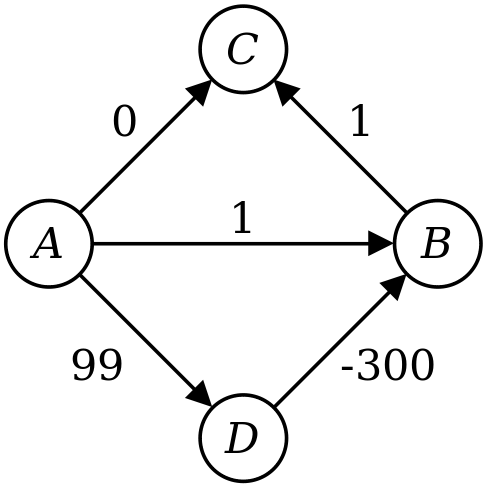
\includegraphics[scale=0.25]{imagenes/wkX2t}

    \href{https://stackoverflow.com/questions/6799172/negative-weights-using-dijkstras-algorithm}{Fuente}
\end{frame}

\begin{frame}{Algoritmo de Dijkstra - Ejercicio}
    El Museo de Experiencias Sensoriales quiere desarrollar un sistema de recomendación en tiempo real que sugiera
    recorridos para visitantes sensibles a distintos tipos de estímulos. cada conexión entre salas tiene un costo
    sensorial de transición. Además, el museo obtiene datos en tiempo real sobre la congestión de cada sala, que
    puede aumentar o disminuir el costo percibido por el visitante (en naranja).

    \begin{adjustbox}{max width=1.1\textwidth, max height=\textheight}
        \begin{tikzpicture}
            \tikzstyle{normal}=[fill=white, draw=black, shape=rectangle];


            % VERTICES
            \node[normal] (Entrada) at (0,0) {Entrada};
            \node[normal] (Luz)      [right=of Entrada] {Luz};
            \node[normal] (Sonido)   [below=of Luz] {Sonido};

            \node[normal] (Digital)  [right=of Luz] {Arte Digital};
            \node[normal] (Zen)      [below=of Digital] {Jardín Zen};

            \node[normal] (Holog)    [right=of Digital] {Hologramas};
            \node[normal] (Oscura)   [below=of Holog, yshift=-1.5cm] {Oscura};

            \node[normal] (Final)    [right=of Holog] {Obra Final};
            \node[normal] (Cine)     [below=of Final] {Cine Inmersivo};

            % Arcos (con costo sensorial)
            \draw[-Latex] (Entrada) -- (Luz)    node[midway, above] {4} node[midway, below] {\orangealert{-1}};
            \draw[-Latex] (Entrada) -- (Sonido) node[midway, below] {7} node[midway, above] {\orangealert{3}};

            \draw[-Latex] (Luz) -- (Digital) node[midway, above] {5} node[midway, below] {\orangealert{0}};
            \draw[-Latex] (Luz) -- (Zen)     node[midway, above] {9} node[midway, below] {\orangealert{-5}};;
            \draw[-Latex] (Luz) -- (Sonido)  node[midway, right] {3} node[midway, left] {\orangealert{-2}};;

            \draw[-Latex] (Sonido) -- (Zen)    node[midway, above] {2} node[midway, below] {\orangealert{1}};
            \draw[-Latex] (Sonido) -- (Oscura) node[midway, below] {6} node[midway, above] {\orangealert{-3}};

            \draw[-Latex] (Digital) -- (Holog)  node[midway, above] {4} node[midway, below] {\orangealert{1}};
            \draw[-Latex] (Digital) -- (Oscura) node[pos=0.8, above] {8} node[pos=0.8, below] {\orangealert{-3}};

            \draw[-Latex] (Zen) -- (Holog) node[midway, above] {3} node[midway, below] {\orangealert{-1}};
            \draw[-Latex] (Zen) -- (Cine)   node[pos=0.75, above] {10} node[pos=0.75, below] {\orangealert{0}};

            \draw[-Latex] (Oscura) -- (Holog) node[pos=0.25, right] {2} node[pos=0.25, left] {\orangealert{2}};
            \draw[-Latex] (Oscura) -- (Cine)   node[midway, below] {5} node[midway, above] {\orangealert{4}};

            \draw[-Latex] (Holog) -- (Final) node[midway, above] {6} node[midway, below] {\orangealert{-2}};
            \draw[-Latex] (Holog) -- (Cine)  node[midway, above] {4} node[midway, below] {\orangealert{1}};

            \draw[-Latex] (Cine) -- (Final) node[midway, right] {3} node[midway, left] {\orangealert{0}};

        \end{tikzpicture}
    \end{adjustbox}

\end{frame}

\begin{frame}{Algoritmo de Dijkstra - Ejercicio}
    \begin{enumerate}
        \item<1-> ¿Cómo buscaríamos un recorrido que minimice el costo?
        \item<2-> ¿Bajo qué supuestos podemos usar Dijkstra?
        \item<3-> ¿Cómo podríamos determinar un recorrido que visite la mayor cantidad de salas con un límite de
        estímulo total $M$?
    \end{enumerate}
\end{frame}
\end{document}